%!TEX root = ../water.tex
% Тип документа
\documentclass[a4paper,12pt]{extarticle}

% Шрифты, кодировки, символьные таблицы, переносы
% \usepackage{cmap}
% \usepackage[T2A]{fontenc}
\usepackage[utf8]{inputenc}
\usepackage[russian]{babel}
% Это пакет -- хитрый пакет, он нужен но не нужен
\usepackage[mode=buildnew]{standalone}

\usepackage
	{
		% Дополнения Американского математического общества (AMS)
		amssymb,
		amsfonts,
		amsmath,
		amsthm,
		% Пакет для физических текстов
		physics,
		% misccorr,
		% 
		% Графики и рисунки
		wrapfig,
		graphicx,
		subcaption,
		float,
		tikz,
		tikz-3dplot,
		caption,
		csvsimple,
		color,
		booktabs,
		geometry,
		% 
		% Таблицы, списки
		makecell,
		multirow,
		indentfirst,
		%
		% Интегралы и прочие обозначения
		ulem,
		esint,
		esdiff,
		% 
		% Колонтитулы
		fancyhdr,
	}  
\usepackage{pgfplots,pgfplotstable,booktabs,colortbl}
\usepackage{xcolor}
\usepackage{hyperref}
\usepackage{gensymb}
\usepackage{textcomp}
\usepackage{pythontex}
\usepackage{qrcode}

\usepackage[e]{esvect} % рисует нормальные вектора

 % Цвета для гиперссылок
\definecolor{linkcolor}{HTML}{000000} % цвет ссылок
\definecolor{urlcolor}{HTML}{799B03} % цвет гиперссылок
 
\hypersetup{pdfstartview=FitH,linkcolor=linkcolor,urlcolor=urlcolor, colorlinks=true}
\hypersetup{pageanchor=false}
% Увеличенный межстрочный интервал, французские пробелы
\linespread{1.3} 
\frenchspacing 

 
% \usetikzlibrary
% 	{
% 		decorations.pathreplacing,
% 		decorations.pathmorphing,
% 		patterns,
% 		calc,
% 		scopes,
% 		arrows,
% 		fadings,
% 		through,
% 		shapes.misc,
% 		arrows.meta,
% 		3d,
% 		quotes,
% 		angles,
% 		babel
% 	}
% Среднее <#1>
\newcommand{\mean}[1]{\langle#1\rangle}
% const прямым шрифтом
\newcommand\ct[1]{\text{\rmfamily\upshape #1}}
\newcommand*{\const}{\ct{const}}
\usepackage{array}
\usepackage{pstool}

\geometry		
	{
		left			=	2.5cm,
		right 			=	1.5cm,
		top 			=	2cm,
		bottom 			=	2cm,
		bindingoffset	=	0cm
	}

%%%%%%%%%%%%%%%%%%%%%%%%%%%%%%%%%%%%%%%%%%%%%%%%%%%%%%%%%%%%%%%%%%%%%%%%%%%%%%%
	%применим колонтитул к стилю страницы
\pagestyle{fancy} 
	%очистим "шапку" страницы
% \fancyhead{} 
	%слева сверху на четных и справа на нечетных
\fancyhead[R]{}%\labauthors 
	%справа сверху на четных и слева на нечетных
% \fancyhead[L]{Отчёт по лабораторной работе №\labnumber}
\fancyhead[L]{\labtheme} 
	%очистим "подвал" страницы
% \fancyfoot{} 
	% номер страницы в нижнем колинтуле в центре
\fancyfoot[C]{\thepage} 

%%%%%%%%%%%%%%%%%%%%%%%%%%%%%%%%%%%%%%%%%%%%%%%%%%%%%%%%%%%%%%%%%%%%%%%%%%%%%%%

\renewcommand{\contentsname}{Оглавление}
\usepackage{tocloft}
\usepackage{secdot}
\sectiondot{subsection}
\usepackage{gensymb}
\usepackage{textcomp}
\usepackage{pythontex}
\usepackage[e]{esvect} % рисует нормальные вектора
\begin{document}
\def\labauthors{Понур К.А.}
\def\labgroup{430}
\def\department{}
% \def\labnumber{1}
\def\labtheme{Численное моделирование морской поверхности}

\renewcommand{\Re}{\operatorname{Re}}
\renewcommand{\Im}{\operatorname{Im}}
\renewcommand{\phi}{\varphi}
\renewcommand{\hat}{\widehat}
\renewcommand{\vec}{\vv}
%!TEX root = ../water.tex
\begin{titlepage}

\begin{center}

{\small\textsc{Федеральное государственное автономное образовательное учреждение\\
высшего образования\\
«Национальный исследовательский\\
Нижегородский государственный университет им. Н.И. Лобачевского»}}
% \vskip 1pt \hrule \vskip 3pt
\vfill
{\small\textsc{Радиофизический факультет}}\\
{\small\textsc {Кафедра Общей физики}}
\vfill
{\small\textsc {Направление <<Радиофизика>>}}

{\Large Отчет по практике \vskip 12pt \bfseries \labtheme}

\end{center}

\vfill
	
\begin{flushleft}
	Руководитель практики Караев В.\,Ю. \\
	Выполнил студент 4-го курса бакалавриата \labauthors
\end{flushleft}
	
\vfill
	
\begin{center}
	Нижний Новгород, \today
\end{center}

\end{titlepage}


\tableofcontents
\newpage


\section{Введение}
В настоящее время, существующая измерительная аппаратура не всегда позволяет получить достаточно полное представление о состоянии приповерхностного  слоя океана, поэтому постоянно разрабатываются новые радиолокационные системы. 
Вместе с тем, для решения таких задач, как проверка качества диагностики состояния поверхности океана существующими радиолокаторами, тестирование и разработка алгоритмов восстановления океанографической информации, а также оценка возможностей новых радиолокаторов, вполне естественным является применение более экономных по времени и средствам методов, в частности численного моделирования.  Однако, при моделировании одномерной морской поверхности, как правило, используется сумма большого числа гармоник, что приводит к значительным затратам машинного времени.

В связи с этим возникает необходимость в минимизации числа гармоник в спектре моделируемой морской поверхности при сохранении необходимой точности при решении различных задач оптики морской поверхности. Здесь возникает ряд нетривиальных вопросов об оптимальном разбиении частотной плоскости на участки и выборе оптимального положения дискретных спектральных компонент в пределах этих участков. Поиску ответов на эти вопросы и посвящена данная работа.


	% Статистическая оптика морской поверхности в настоящее время представляет собой самостоятельную и бурно развивающуюся область оптики моря. Она включает  в себя ряд важных и интересных проблем, основной из которых является изучение статистических характеристик над- и подводных световых полей, созданных как естественными, так и искуственными источниками при наличии случайно-неровной границы раздела воздух-вода. 

	% Разработанные к настоящему времени теоретические методы расчета световых полей в море при наличии ветрового волнения на поверхности в основном строятся на геометроортическом описании распространения световых лучей и использовании результатов решения уравнения переноса излучения в рассеивающих средах. Эти методы, как правило, позволяют исследовать статистические моменты лишь первого и второго порядков, причём вычисление последних часто наталкивается, особенно при учёте эффектов двукратного прохождения излучения через морскую поверхность , на существенные и даже порой непреодолимые трудности. Это заставляет исследователей идти по пути упрощения или идеализации как моделей формирования световых полей, так и модели волнения на поверхности раздела. Однако, результаты , полученные в рамках приближенных моделей, могут оказаться не вполне соответствующими действительности и поэтому нуждаются в проверке.



% \section{Цель}

% \section{Формулы для спектров и корреляционных функция волнения}
\section{Небольшое введение в корреляционную теорию}
Рассмотрим ряд общих понятий, описывающих возвышения и уклоны взволнованной морской поверхности в рамках теории случайных пространственно-временных полей. Представим возвышения поверхности в виде суммы гармонических бегущих волн с независимыми (случайными) фазами:
\begin{equation}
	\label{eq:1}
	\zeta(\vec r, t)=\Re \iint\limits_{\infty} \dd{\dot \zeta(k)} \exp{i(\vec k \vec r - \omega_k t)}, 
\end{equation}
где $\dd{\dot \zeta}$ -- комплексная амплитуда гармоники с волновым числом $\vec k$  и временной частотой $\omega_k$, связанной с $\vec k$ дисперсионным соотношением $\omega_k=\sqrt{g k }$, $\vec{k}=\vec{x_0} k_x + \vec{y_0} k_y$, $\rho=\vec{x_0} x + \vec{x_0} y$,
$x_0,y_0$ -- орты декартовой системы координат, $k=\abs{k}$ -- пространственная частота, $t$ -- время, $g=9.81 ~ \frac{\text{м}}{\text{с}^2}$ -- ускорение свободного падения.


Пространственно-временная корреляционная
\footnote{Нужно разобраться с названиями, но судя по всему так далее называется смешанный момент}
 функция возвышений по определяется выражением:
\begin{gather}
\label{eq:2}
	M_{\zeta}(\vec{r_1},\vec{r_2},t_1,t_2)= \mean{\zeta(\vec{r_1},t_1)\zeta(\vec{r_2},t_2) }
\end{gather}
В соответствии с \eqref{eq:1}:
\begin{gather*}
	M_{\zeta}(\vec{r_1},\vec{r_2},t_1,t_2)= \frac12 \Re 
	\iint\limits_{\infty}  \iint\limits_{\infty} 
	\mean{\dd{\dot \zeta(\vec k_1)} \dd{\dot \zeta(\vec k_2)} } 
	\exp{i(\vec k_1 \vec r - \omega_1 t_1 + \vec k_2 \vec r - \omega_1 t_2)} +\\ 
	+\mean{\dd{\dot \zeta(\vec k_1)} \dd{\dot \zeta^*(\vec k_2)} } 
	\exp{i(\vec k_1 \vec r - \omega_1 t_1 - \vec k_2 \vec r + \omega_1 t_2)}
\end{gather*}

Поскольку двумерная плотность вероятности стационарного процесса зависит от $t_1$ и $t_2$ через разность $\tau=t_2-t_1$, то смешанный момент второго порядка будет зависеть только от $\tau$\footnote{доказать}. Аналогично можно сказать и про $\vec r_1$ и $\vec r)2$

Итак, для статически однородного и стационарного поля выполняется соотношение: 
\begin{equation}
	M_{\zeta}(\vec r_1, \vec r_2,t_1,t_2)=M_{\zeta}(\vec \rho= \vec r_2 - \vec r_1, \tau =t_2-t_1)
\end{equation}
Чтобы это соотношение было справедливым в нашей задаче, необходимо потребовать выполнение условий
\begin{equation}
	\frac12 \mean{\dd{\dot \zeta(\vec k_1)} \dd{\dot \zeta(\vec k_2)} } =0 
	~~~\text{ и }~~~ \frac12 \mean{\dd{\dot \zeta(\vec k_1)} \dd{\dot \zeta^*(\vec k_2)} } =
	\tilde S(\vec k_1) \delta(\vec k_2- \vec k_1) \dd{\vec k_1} \dd{\vec{k_2}}.
\end{equation}
где $\tilde S(\vec k)$ -- волновой спектр морской поверхности, $\delta(\vec k_2 - \vec k_1)$ -- дельта-функция. Подставляя эти условия в \eqref{eq:2}, получим:
\begin{equation}
	\label{eq:3}
	M_{\zeta}(\rho, \tau)= \iint\limits_{\infty} S(\vec{k}) \cos(\vec k \vec \rho - \omega_k \tau) \dd{k}.
\end{equation}

Винеровский энергетический спектр определяется преобразованием Винера-Хинчкина функцией корреляции, описываемой \eqref{eq:3}

\begin{gather}
	\label{eq:4}
	\Phi_{\zeta}(\vec k ,\omega)= \iiint\limits_{\infty} 
	M_{\zeta}(\vec \rho, \tau) e^{-i\qty(\vec k \vec \rho + \omega t)} \dd{\rho} \dd{\tau}=4\pi^3 \qty[\tilde S(\vec k) \delta(\omega+\omega_k)+\tilde S(- \vec k) \delta(\omega- \omega_k)].
\end{gather}
Из \eqref{eq:4} следуют, как частные случаи, выражения для пространственного,
\begin{equation}
	\Phi_{\zeta}(\vec k)=\frac{1}{2\pi} \int\limits_{\infty} \Phi_{\zeta}(\vec k, \omega) \dd{\omega}= 2 \pi^2 \qty[\tilde S(\vec k)+\tilde S(-\vec k)],
\end{equation}
и временного спектров Винера.

{\color{red}{Разобрать фундаментально всю  теорию до этого момента.}}
\section{Реальное и модельное поля уклонов волнения}

Обратимся сначала к задаче моделирования случайного одномерного поля уклонов взволнованной поверхности. 

Представим модельное поле уклонов в виде суммы N синусоид с детерминированными амплитудами $a_i$ и случайными фазами $\varphi_i$:
\begin{equation}
	\Sigma(r)=\sum_{i=1}^N a_i \sin(k_ir+\varphi_i), 
\end{equation}
где $b_i=\frac{a_i^2}{2}$.

Допустим что величины $k_i$ не находятся в дробно-рациональных отношениях друг к другу. В этом случае можно полагать, что сложение гармонических составляющих с частотами $k_i$ и амплитудами $b_i$ при больших $\rho$ происходит <<некогерентным>> образом. При этом мощность <<шума>> функции $\tilde M_q(\rho)$ определяется выражением 
$\displaystyle \sigma^2= \sum_{i=1}^N \frac{b_i^2}{2}$. В области малых $\rho$, напротив, гармоники суммируются <<когерентно>> и соответствующая <<мощность>> равна 
$\displaystyle \tilde M^2_q(0)=\qty(\sum_{i=1}^N b_i)^2$. Образуем величину 
$Q=\sigma^2/\tilde M_q(0)$, которая характеризует относительную мощность шумов. Минимум этой величины находится путём решения системы уравнений $\pdv{Q}{b_i}=0$, для $i=1,2,\dots,N.$
Результатом её решения является $b_1=b_2=\dots = d_N$. Спектр модельного поля при этом имеет близкий к белому вид, а выравнивание амплитуд спектральных компонент реального поля $S_q$ сводится к разбиению области определения спектра $[0, k_m]$ на участки $\Delta k_i$, интегралы по которым от функции $S_q(k)$ имеют одно и то же значения $b_i=b_0=\sigma^2_q/N$.

Заметим теперь, что, рассуждая о способах разбиения интервала частот $[0, k_m]$ на участки $\Delta k_i$, мы оставляли нерешенным вопрос о выборе собственно узлов спектра $k_i$ внутри этих участков. Обычно узел $k_i$ ставится у правой границы ячейки $\Delta k_i$. При этом, однако, оказывается, что модельная корреляционная функция плохо согласуется с реальной корреляционной функцией в области малых $\rho$. Для достижения такого согласия следует потребовать сопряжения всех производных (от первого до $N$-о порядка) функция $\tilde M_q(\rho)$ и $M_q(q)$ при $\rho=0$. Это условие эквивалентно требованию сопряжения моментов спектров модельного и реального полей уклонов, которое записывается в виде 
\begin{equation}
	\sum_{i=1}^N b_ik_i^{2p}=\int\limits_{0}^{\infty} k^{2p}S_q(k)k\dd{k},
\end{equation}
для $p=1,2,\dots,N.$

Полученная система N уравнений для N неизвестных $k_i$ не имеет общего решения и потому может анализироваться лишь численно, что тоже связано со значительными сложностями.

Оставим пока эту задачу за рамками данной работы.

Наиболее простое решение вопроса о выборе узлов заключается в том, чтобы потребовать выполнения облегченного, по сравнению с предыдущим, условия сопряжения вторых моментов модельного и реального спектров уклонов:
\begin{equation}
	b_i k_i^2=\int\limits_{\Delta k_i} k^2 S_q(k) k \dd{k}.
\end{equation}

Из него непосредственно следует правило нахождения узлов $k_i$. В частности, получаем
\begin{equation}
	k_i=\sqrt\frac{1}{b_0} \int\limits_{\Delta k_i} k^2 S_q(k) k \dd{k}.
\end{equation}

Такой способ выбора узлом, как нетрудно убедиться, обеспечивает сопряжения корреляционных функция реального и модельного полей по второй производной в нуле, или, иначе говоря, равенство дисперсий кривизн этих полей, что весьма важно при решении многих задач оптики морской поверхности:

\section{Корреляционные функции высот и уклонов}

\begin{figure}[h!]
\begin{minipage}[h]{0.45\linewidth}
	\centering
	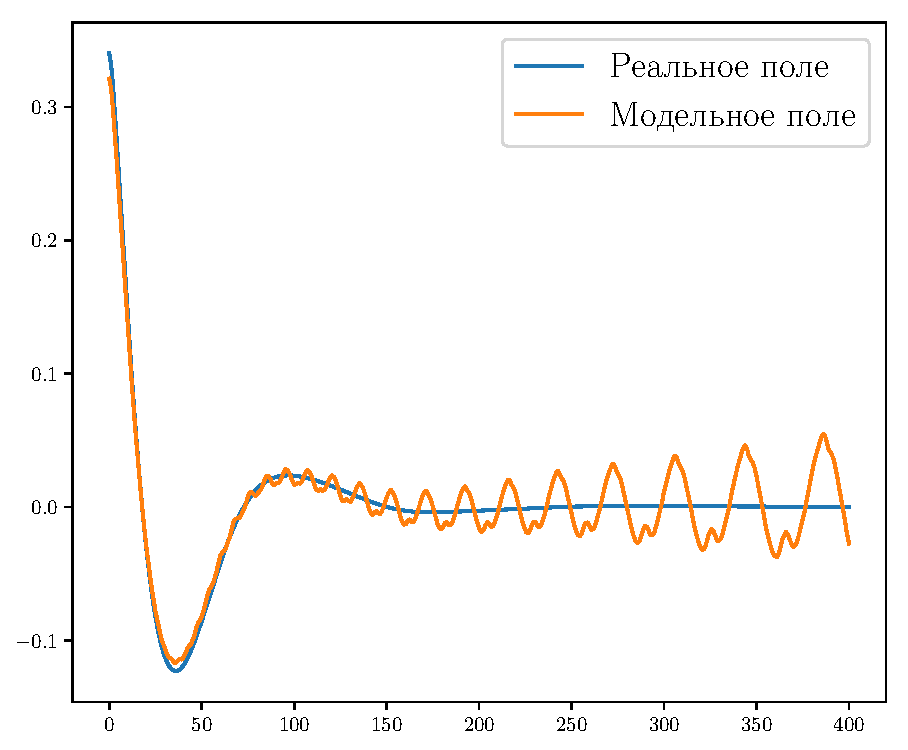
\includegraphics[width=\linewidth]{fig/correlation_hlog_100.pdf}
	\caption{Корреляционная функция высот при расположении узлов, равномерно распределенных в логарифмическом масштабе. $N=100, ~U_{10}=10$.}
	\label{fig:cor_h_b}
\end{minipage}
\hfill
\begin{minipage}[h]{0.45\linewidth}
	\centering
	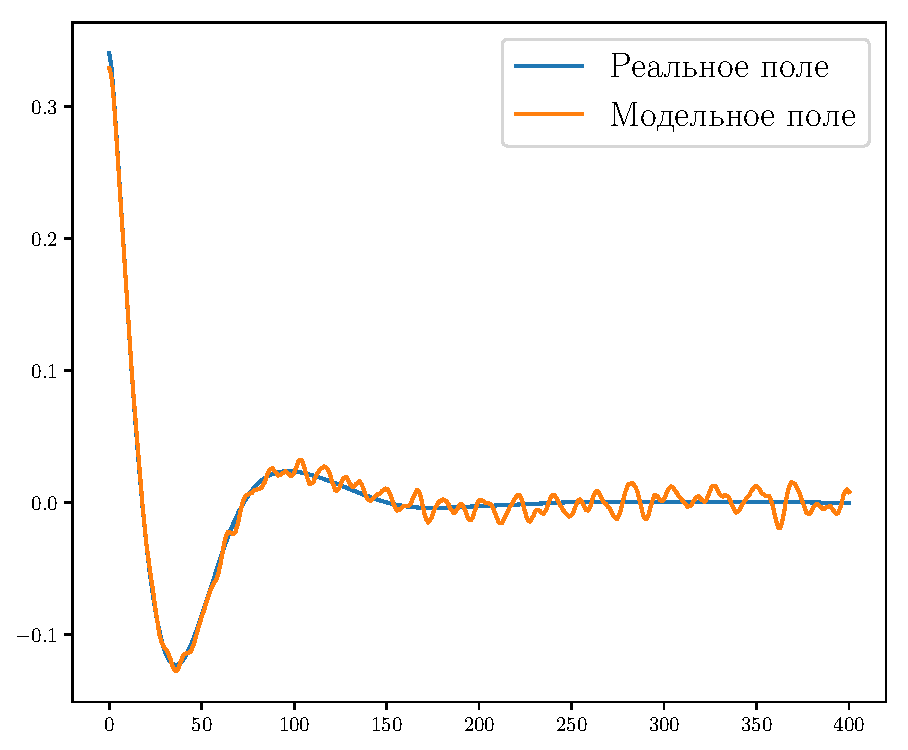
\includegraphics[width=\linewidth]{fig/correlation_hwn_100.pdf}
	\caption{Корреляционная функция высот при расположении узлов по методу <<отбеливания спектра>>. $N=100, ~U_{10}=10$.}
	\label{fig:cor_h_a}
\end{minipage}
\end{figure}


% \begin{figure}[h!]
% \begin{minipage}[h]{0.45\linewidth}
% 	\centering
% 	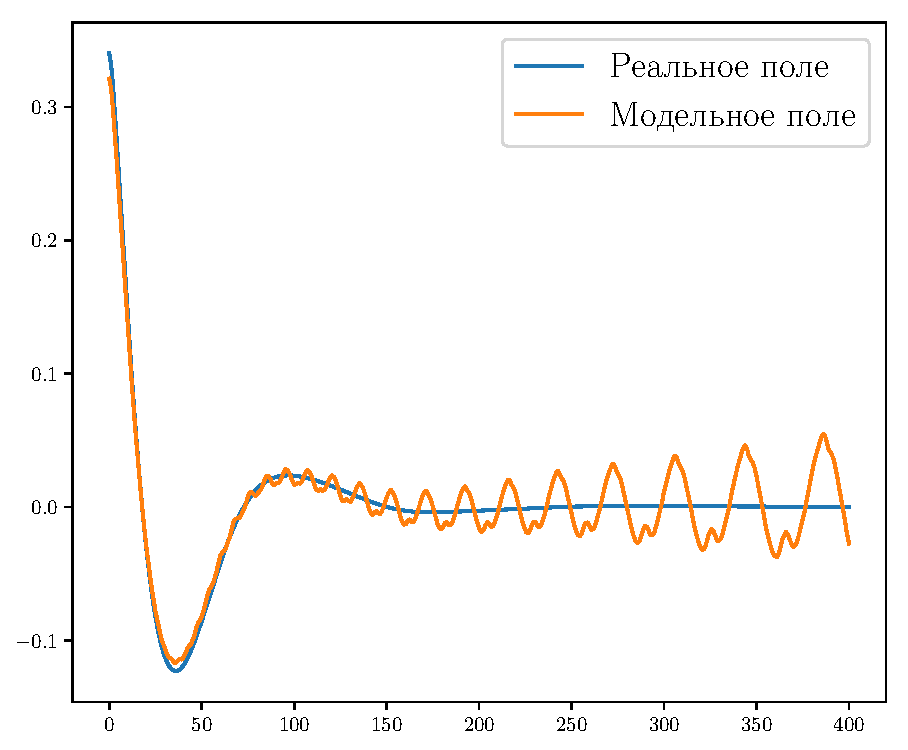
\includegraphics[width=\linewidth]{fig/correlation_hlog_100.pdf}
% 	\caption{Корреляционная функция высот при расположении узлов, равномерно распределенных в логарифмическом масштабе. $N=100, ~U_{10}=10$.}
% 	\label{fig:cor_h_b}
% \end{minipage}
% \hfill
% \begin{minipage}[h]{0.45\linewidth}
% 	\centering
% 	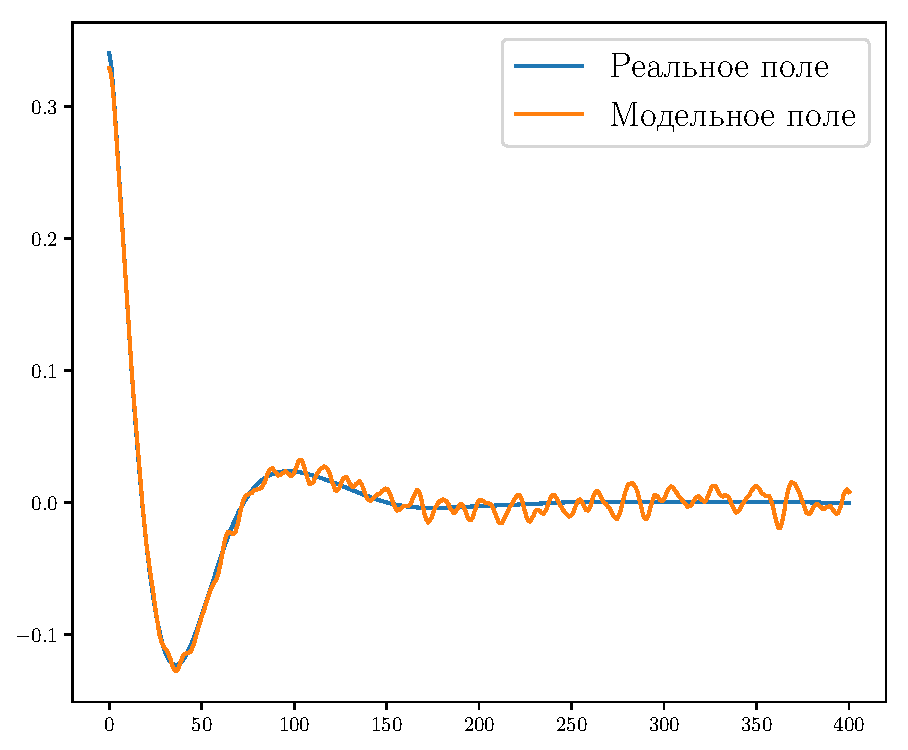
\includegraphics[width=\linewidth]{fig/correlation_hwn_100.pdf}
% 	\caption{Корреляционная функция высот при расположении узлов по методу <<отбеливания спектра>>. $N=100, ~U_{10}=10$.}
% 	\label{fig:cor_h_a}
% \end{minipage}
% \end{figure}


\section{Заключение}
\begin{figure}[h!]
\begin{minipage}[h]{0.45\linewidth}
	\centering
	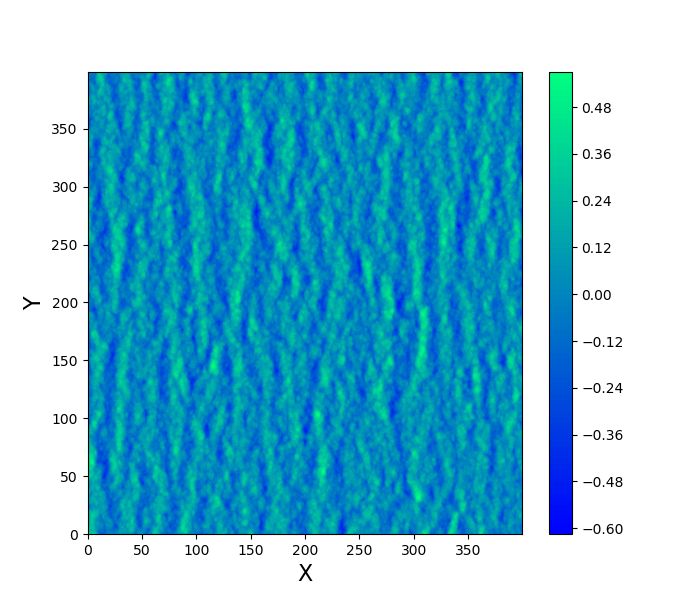
\includegraphics[width=\linewidth]{img/water5.png}
	\caption{Моделирование высот морского волнения. $N=1000, ~ U_{10}=5$ }
	\label{fig:water5}
\end{minipage}
\hfill
\begin{minipage}[h]{0.45\linewidth}
	\centering
	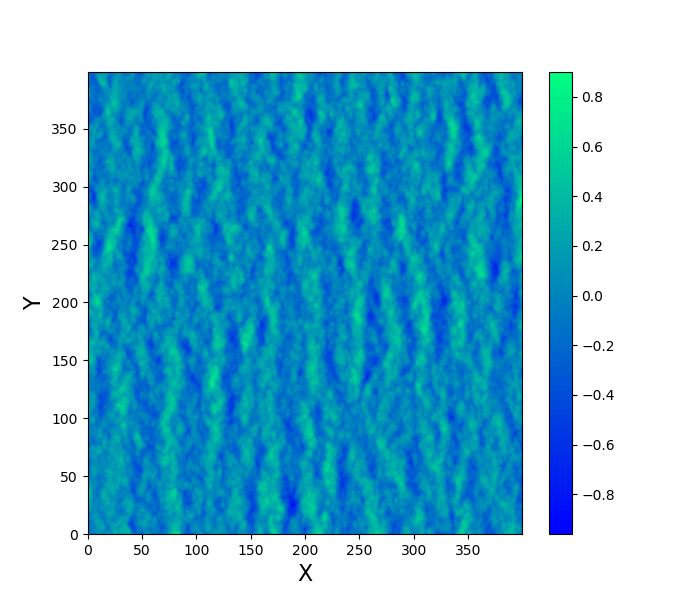
\includegraphics[width=\linewidth]{img/water6.png}
	\caption{Моделирование высот морского волнения. $N=1000, ~ U_{10}=6$ }
	\label{fig:water6}
\end{minipage}

\vfill
\begin{minipage}[h]{0.45\linewidth}
	\centering
	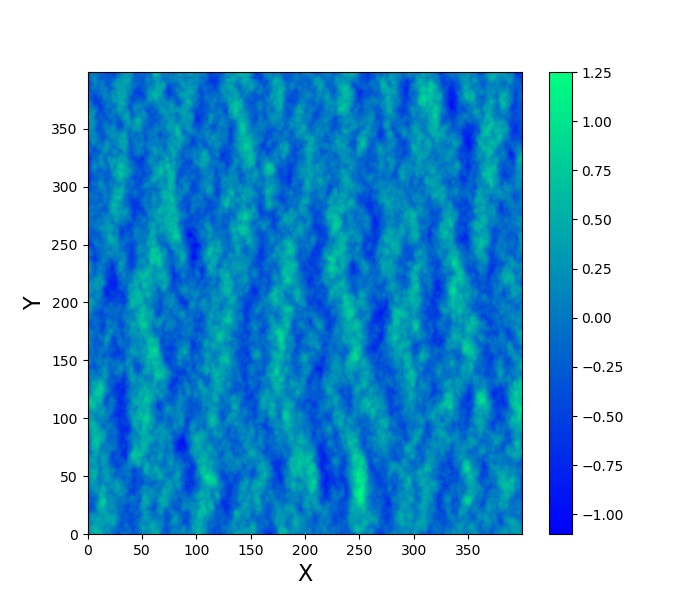
\includegraphics[width=\linewidth]{img/water7.png}
	\caption{Моделирование высот морского волнения. $N=1000, ~ U_{10}=7$  }
	\label{fig:water7}
\end{minipage}
\hfill
\begin{minipage}[h]{0.45\linewidth}
	\centering
	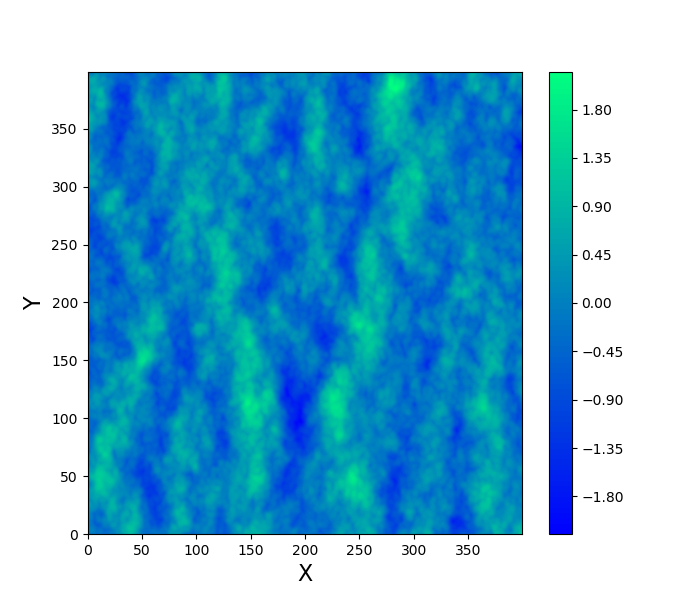
\includegraphics[width=\linewidth]{img/water10.png}
	\caption{Моделирование высот морского волнения. $N=1000, ~ U_{10}=10$ }
	\label{fig:water10}
\end{minipage}
\end{figure}



\section{Моделирование волнения}
\label{model}
\subsection{Модель спектра волнения}

Для моделирования волнения используется следующая модель спектра волнения, предложенного в \cite{Karaev2}: 
\begin{equation}
	\label{eq:Sw}
	\begin{cases}
		S(\omega)=S_J(\omega), &  0<\omega\leq 1.2\,\omega_m\\
		S(\omega)= \frac{\alpha_2}{\omega^4}, &  1.2 \,\omega_m < \omega \leq \alpha_m \omega_m\\
		S(\omega)= \frac{\alpha_3}{\omega^5}, &   \alpha_m \omega_m< \omega \leq \omega_gk\\
		S(\omega)= \frac{\alpha_4}{\omega^{2.7}}, & \omega_{gk}<\omega\leq \omega_h\\
		S(\omega)= \frac{\alpha_5}{\omega^5}, & \omega_h<\omega,
	\end{cases}
\end{equation}
где коэффициенты $\alpha_i$ задаются следующим образом:
\begin{equation}
	\label{eq:alpha_i}
	\begin{cases}
		\alpha_2=S_J(1.2 \omega_m)\cdot (1.2 \omega_m)^4 \\
		\alpha_3=a_2\cdot \alpha_m \omega_m \\
		\alpha_4= \frac{\alpha_3}{\omega^{2.3}_{gk}} \\
		\alpha_5 = \alpha_4 \cdot \omega_h^{2.3} \\
		\alpha_m = f(U_{10}), & 
	\end{cases}
\end{equation}
$U_{10} \text{-- скорость ветра на высоте 10 метров над уровнем моря,}$ а $S_J(\omega)$-- спектр JONSWAP:
\begin{equation}
\label{eq:Sj}
	S_J(\omega)\sim \frac{g^2}{\omega^{5}}\exp{-\qty(\frac{\omega_m}{\omega})^4}
	\cdot \gamma^{\exp{-\omega^2}}
\end{equation}
Стоит отметить, что в конечном счете формулы \eqref{eq:Sw},\eqref{eq:alpha_i},\eqref{eq:Sj} в модели использовались в $k-$представлении, т.е.  был выполнен переход $S(\omega)\rightarrow S(k)$

\begin{figure}[h!]
	\centering
	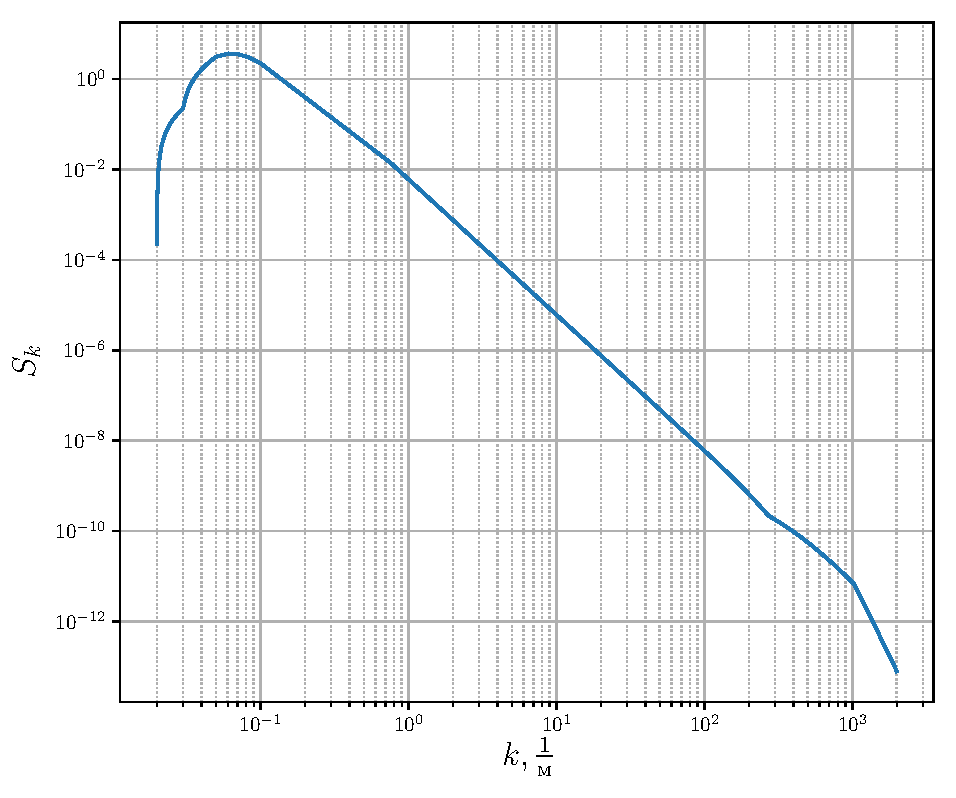
\includegraphics[width=0.7\linewidth]{fig/full_spectrum}
	\caption{Используемая модель спектра волнения в k-представлении. 
	Параметры: $\tilde x=20170, U_{10}=10 \frac{\text{м}}{\text{с}}$}
	\label{fig:full_spectrum}
\end{figure}
\subsection{Модель углового распределения}
Угловое распределение $\Phi_{\omega}$ в данной работе описывается следующей формулой:
\begin{equation}
	\Phi_{k} (k, \phi)= A\cdot \cosh^{-1}{2B(k) \phi}, ~~ -\pi\leq \phi \leq \pi,
\end{equation}
где $\phi=\phi_m = \phi_w$, $\phi_w$-- генеральное направление распространения волнения,
$\phi_m$-- текущий азимутальный угол, $A$-- нормировочный коэффициент.


\begin{figure}[h!]
	\centering
	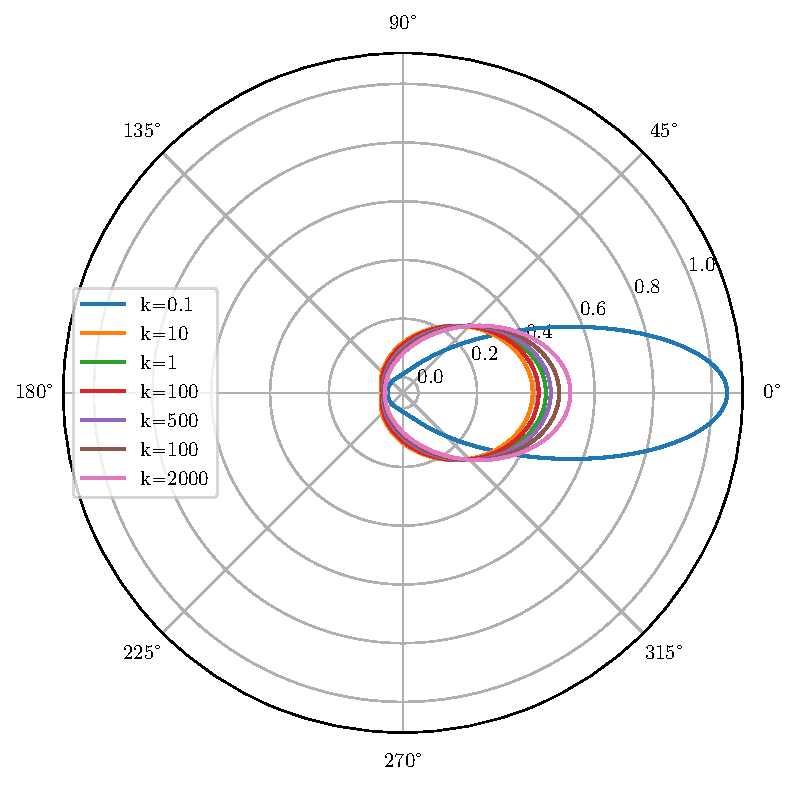
\includegraphics[width=0.7\linewidth]{fig/full_angles}
	\caption{Используемая модель  углового распределения для различных значений $k$. 
	Параметры: $\tilde x=20170, U_{10}=10 \frac{\text{м}}{\text{с}}$}
	\label{fig:full_spectrum}
\end{figure}


Дисперсионное уравнение в данной работе имеет вид:
\begin{equation}
	\label{eq:w_k}
	\omega(k)=\sqrt{gk+a\cdot k^3},
\end{equation}
Значения и физический смысл всех коэффициентов можно найти в \cite{Karaev1}, а также в исходном коде программы 
(\href{https://github.com/KirillPonur/water}{github.com/KirillPonur/water})

\newpage
\begin{thebibliography}{}
	\bibitem{Karaev1} \textit{В.Ю.Караев, М.Б. Каневский, Г.Н. Баландина}, Численное моделирование поверхностного волнения и дистанционное зондирование // Препринт №552 ИПФ РАН, 2002, С.1-10.
	\bibitem{Veber} \textit{В.Л. Вебер}, О моделировании случайного профиля морской поверхности // Изв. вузов. Радиофизика. 2017. Т. 60, № 4. С. 346.
	\bibitem{Karaev2} \textit{В.Ю.Караев, Г.Н. Баландина} Модифицированный спектр волнения и дистанционное зондирование // Исследование Земли из космоса, 2000, N5, C.1-12.
\end{thebibliography}
\textbf{Примечание.} Модель написала на языке Python с использованием библиотек NumPy и SciPy, курсовая и презентация к ней оформлены в издательской системе \LaTeX\,с использованием пакета Beamer. Актуальную версию программы можно найти на 
Github'e: (\href{https://github.com/KirillPonur/water}{github.com/KirillPonur/water})
\end{document}